\section{Implementation und Test des ersten Prototyp}\label{sec:pro1}

\subsection{Implementation}
In Kapitel 5 wurden, in Bezug auf die Evaluationsergebnisse aus dem vorherigen Kapitel, Umsetzungsmöglichkeiten für die verschiedenen Nielsen-Heuristiken herausgearbeitet.
Diese sollen in die Implementierung des ersten Prototyp einfließen, und so für eine guten Grundstein für eine positive Benutzererfahrung der App sorgen. \\

Der erste Prototyp wurde am 16. Dezember 2017 in Form einer Android-Library fertiggestellt, auf \emph{JitPack.io}, einem online Service zum Verwalten und Teilen von Android-Projekten, hochgeladen, und so in die bestehende Android-App als Bibliothek eingebunden. \\
\todo{Hier bild von buid.gralde?}

Bei der Implementierung wurde das Entwurfsmuster des \emph{Model-View-Controllers} eingesetzt, welches den Quellcode in drei verschiedene Komponente unterteilt (siehe \autoref{fig:mvc}).
So gibt es einerseits das \emph{Datenmodell (model)}, die \emph{Präsentationskomponente (view)} und die \emph{Programmsteuerung (controller)}.
Ziel dieses Musters ist es, eine flexible Architektur zu schaffen, die bei Bedarf leicht erweitert bzw. wiederverwendet werden kann.

\begin{figure}[h]
  \centering
  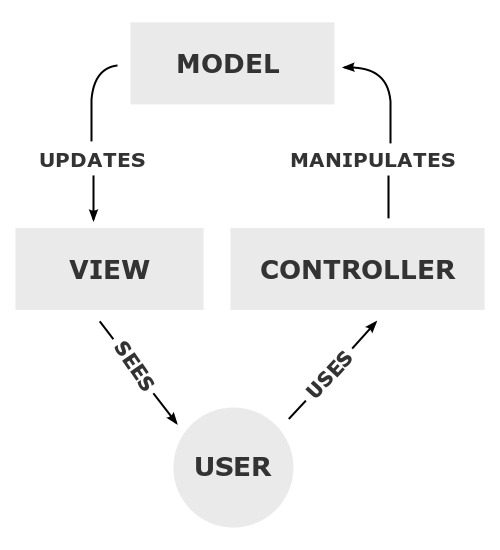
\includegraphics[keepaspectratio, width=0.5\textwidth]{mvc}
  \caption{Interaktion innerhalb des Model-View-Controller Prinzips}
  \label{fig:mvc}
\end{figure}

\noindent
Zusätzlich wurde der Aufbau des Projekts in der \emph{Unified Modelling Language}, kurz \emph{UML}, modelliert.
Dies ermöglicht bereits vor der eigentlichen Implementierung wichtige Begriffe und mögliche Beziehungen festzulegen, und einen Überblick über die benötigten Klassen zu bekommen.
Die Komponente des \emph{Datenmodells} sah dabei wie folgt aus (die beiden weiteren Komponenten befinden sich im Anhang):

\begin{figure}[h]
  \centering
  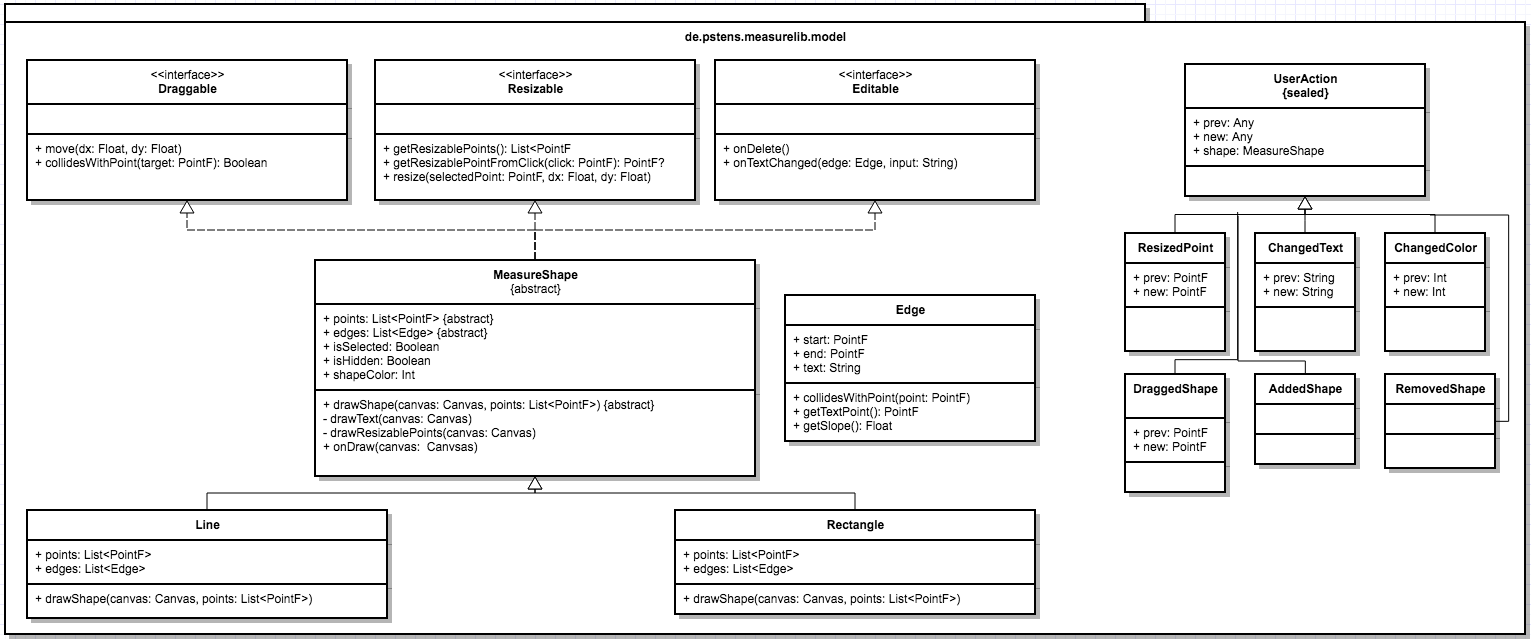
\includegraphics[keepaspectratio, width=\textwidth]{prototype1/model}
  \caption{Datenmodell-Komponente als UML-Diagramm}
  \label{fig:model1}
\end{figure}

\noindent
In \autoref{fig:model1} ist zentral die abstrakte Klasse \emph{MeasureShape} zu erkennen, welche die Oberklasse der beiden Formen \emph{Line} und \emph{Rectangle} ist.
Diese vererbt die abstrakten Attribute \emph{points} und \emph{edges} an die Unterklassen, welche diese in ihrer Implementierung überschreiben müssen.
Außerdem muss jeweils die öffentliche Methode \emph{drawShape(...)} implementiert werden.
Dies sorgt dafür, dass jede Unterklasse selber dafür verantwortlich ist, wohin und wie ihre Form gezeichnet wird. 
\emph{MeasureShape} selber implementiert drei verschiedene \emph{Interfaces}, die diverse Methoden zum Verschieben, Vergrößern und Editieren für alle ihre Unterklassen bereit stellen. \\

\noindent
Eine weitere Klasse in dem \emph{Datenmodell} ist \emph{UserAction}.
Diese ist eine versiegelte (\emph{sealed}) Oberklasse, welche die verschiedenen Aktionen, die der Nutzer ausführen kann, darstellt.
Versiegelt bedeutet in diesem Kontext, dass nur Klassen, welche im \emph{Scope} der Oberklasse liegen, von dieser erben können.
In diesem ersten Prototyp unterstützt die App das Wiederholen bzw. rückgängig machen von den folgenden sechs Aktionen: 

\begin{itemize}
  \item Verschieben von Formen (\emph{DraggedShape})
  \item Hinzufügen von Formen (\emph{AddedShape})
  \item Löschen von Formen (\emph{RemovedShape})
  \item Vergrößern bzw. verkleinern von Formen (\emph{ResizedPoint})
  \item Ändern des Textes (\emph{ChangedText})
  \item Ändern der Farbe (\emph{ChangedColor})
\end{itemize}

\noindent
Funktional beschränkt sich die Implementierung des ersten Prototyps zunächst auf das Zeichnen von einfachen Linien und Vierecken, sowie das anschließende Beschriften dieser, um Messwerte einzutragen. \\

Dabei wurde eine Zoom-Linse (siehe \autoref{fig:draw1}), wie sie bei allen drei Applikationen aus Kapitel 4 umgesetzt wurde, zum schnelleren und einfacheren Einzeichnen von Formen benutzt. \\

Das Wechseln des Modus ist über einen \emph{Floating Action Button} im unteren rechten Bereich des Bildschirms möglich (siehe \autoref{fig:all1}).
Zudem kann der Benutzer über einen weiteren \emph{Floating Action Button} im unteren linken Bildschirmbereich jederzeit ein neues Bild aufnehmen, oder ein bereits vorhandenen importieren. \\

Undo- sowie Redo-Funktion wurden auf dedizierte \emph{Buttons} in die obere Menüleiste gelegt.
Hier gibt es außerdem jeweils einen Button, um ausgewählte Formen zu löschen, die Zeichenfarbe zu ändern, oder eine andere Form zum Zeichnen auszuwählen. \\

\begin{figure}[h]
  \begin{subfigure}[t]{0.4\textwidth}
    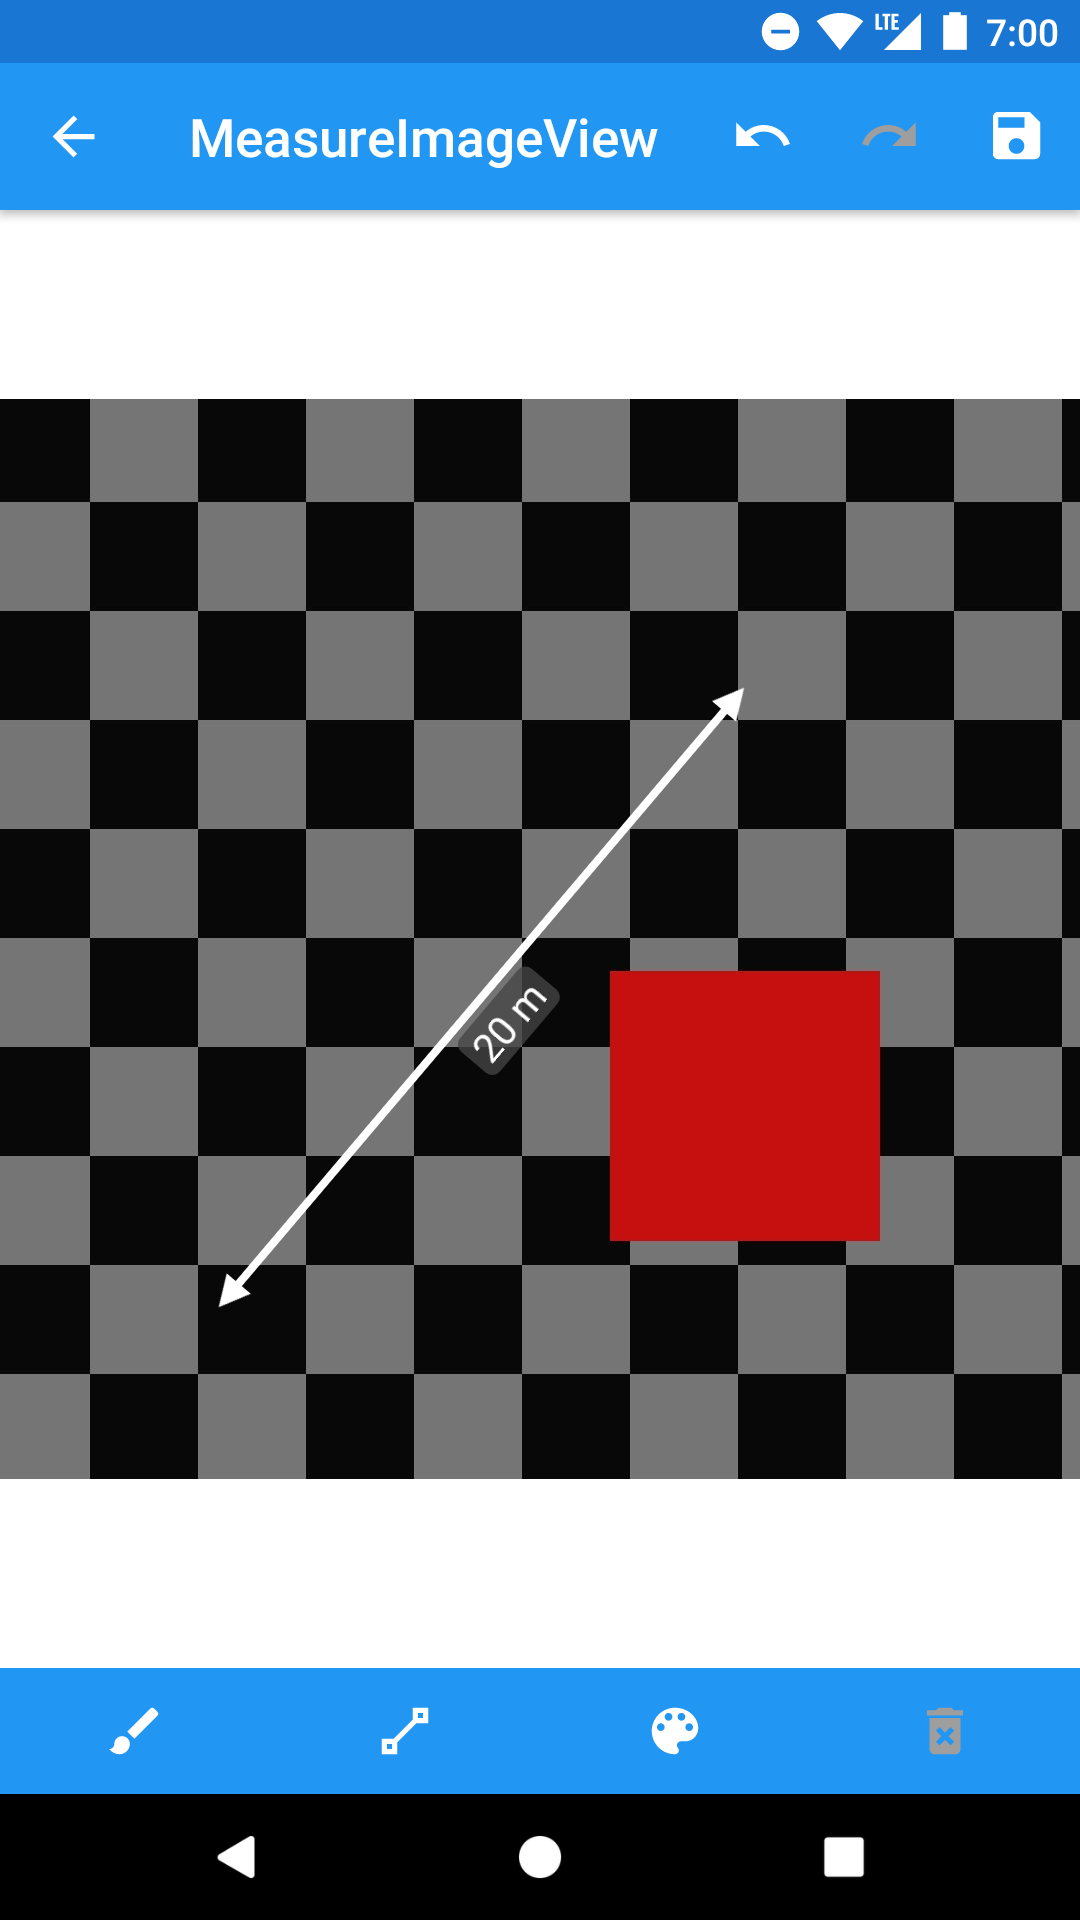
\includegraphics[keepaspectratio, width=\textwidth]{prototype1/all}
    \caption{Erster Prototyp mit bereits eingezeichneter Linie}
    \label{fig:all1}
  \end{subfigure}
  \begin{subfigure}[t]{0.4\textwidth}
    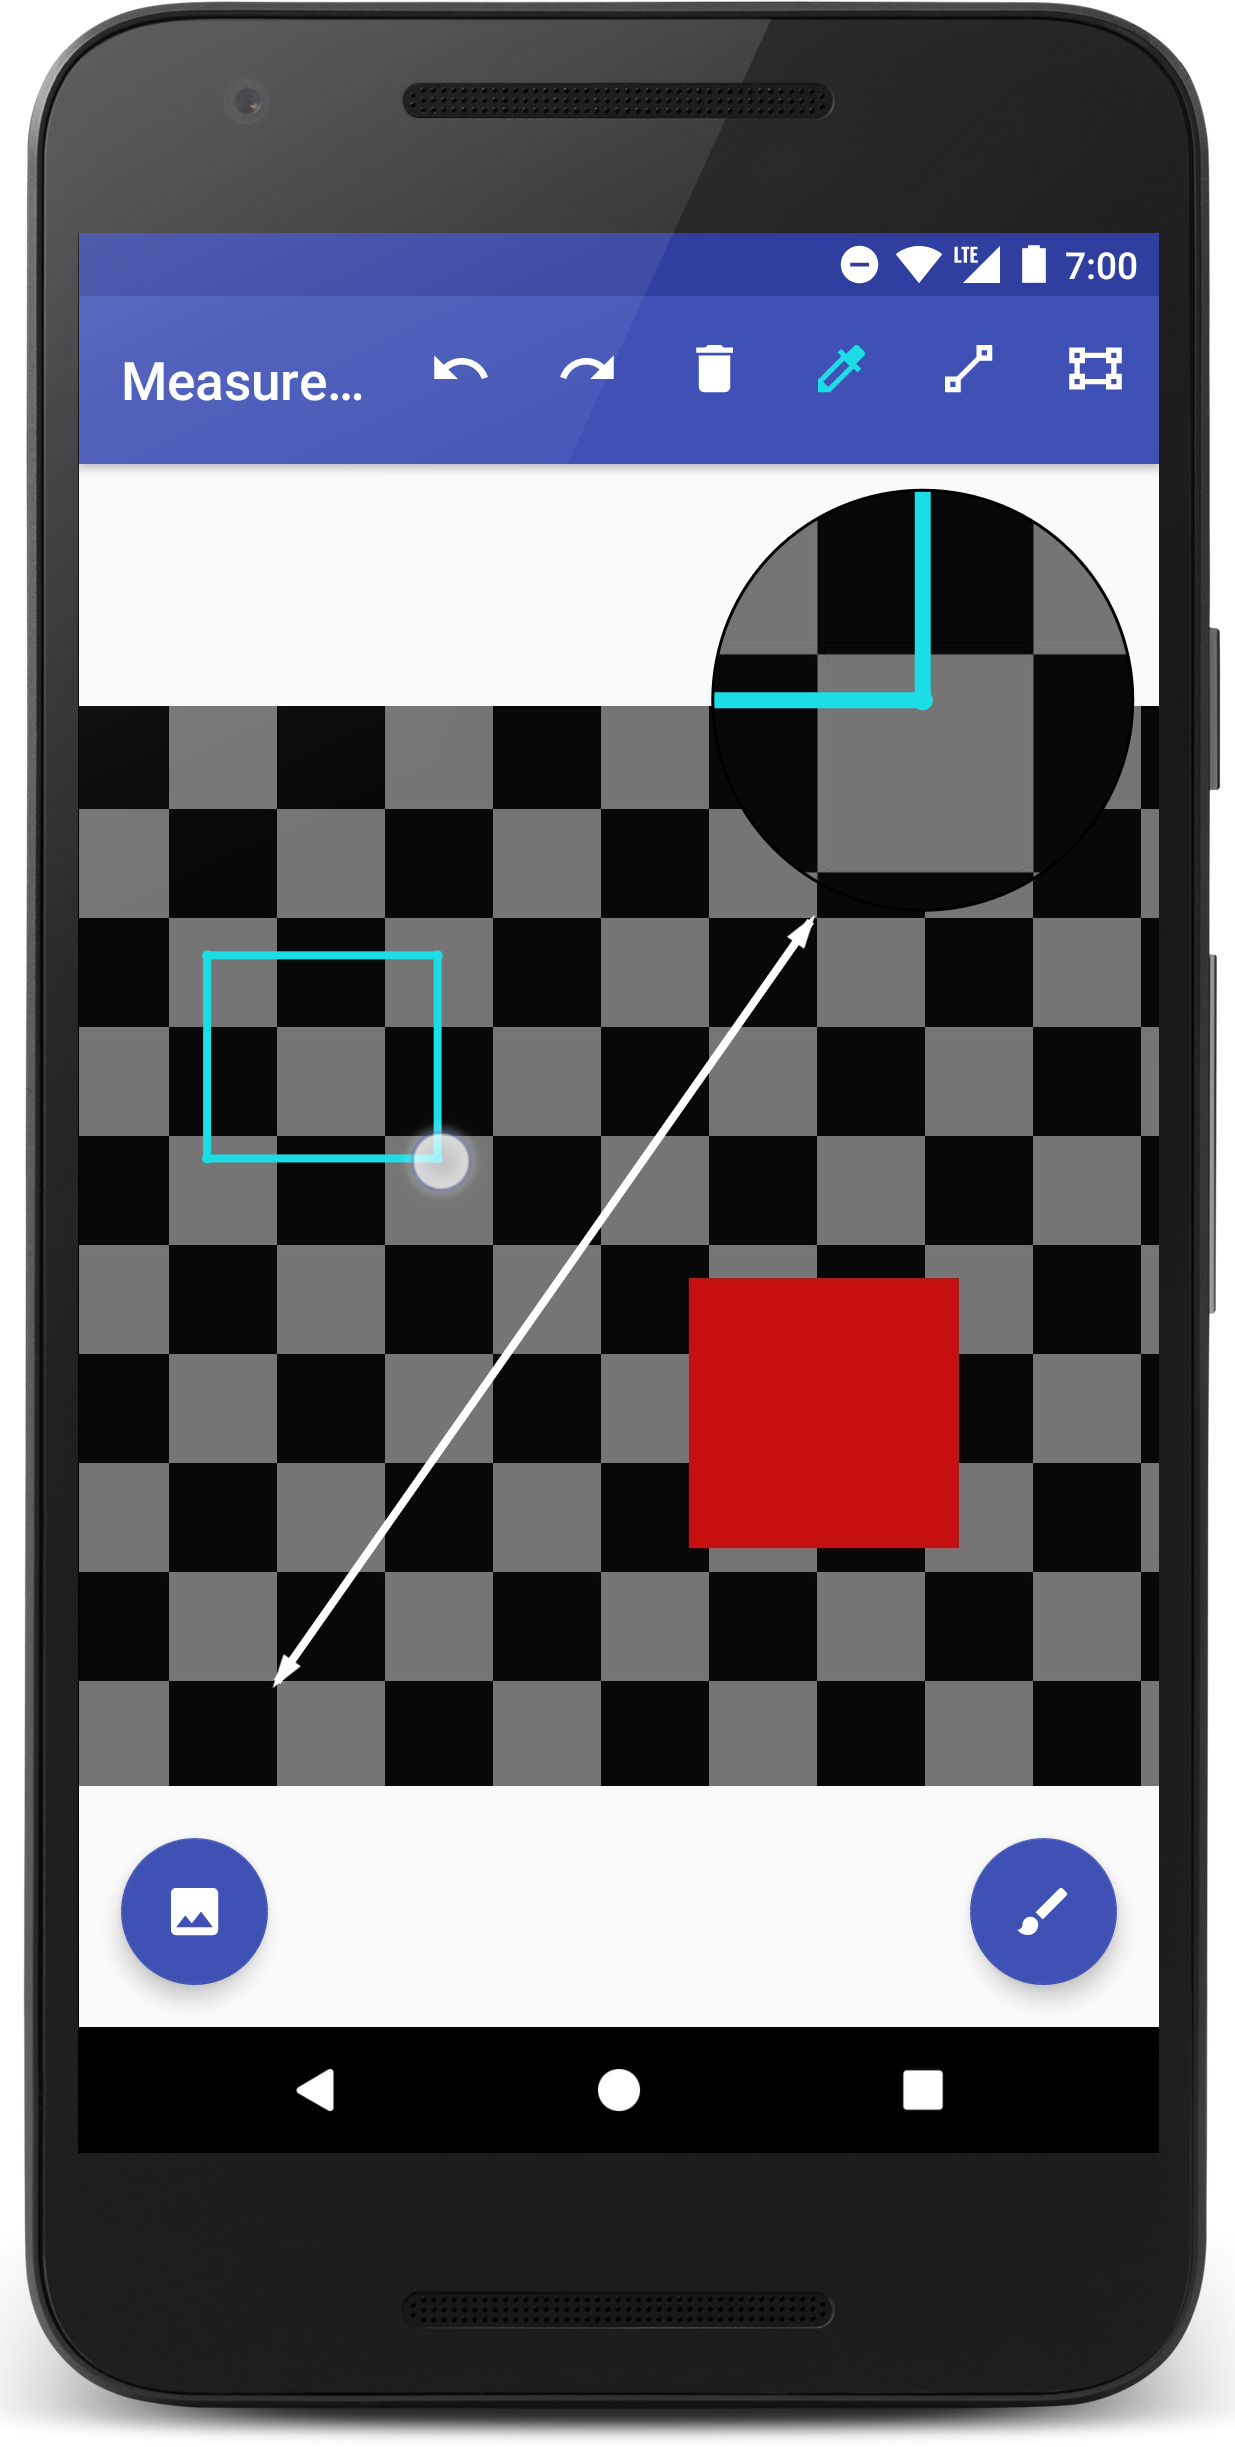
\includegraphics[keepaspectratio, width=\textwidth]{prototype1/drawing}
    \caption{Zoom-Linse beim Zeichnen einen Vierecks}
    \label{fig:draw1}
  \end{subfigure}
  \centering
  \caption{Erster Prototyp bei eingezeichneter Linie und beim Zeichnen eines Vierecks}
\end{figure}

\noindent
Beim Auswählen des Farb-Icons in der Menü-Leiste öffnet sich ein modaler Dialog, der es dem Benutzer ermöglicht, aus einem Farbkreis die gewünschte Farbe auszuwählen (siehe \autoref{fig:color1}).
Diese Farbe wird für alle neu eingezeichneten Formen standardmäßig benutzt.
Falls zuvor eine Form markiert wurde, wird diese ebenfalls mit der ausgewählten Farbe eingefärbt. \\

\begin{wrapfigure}{R}{0.5\textwidth}
  \centering
  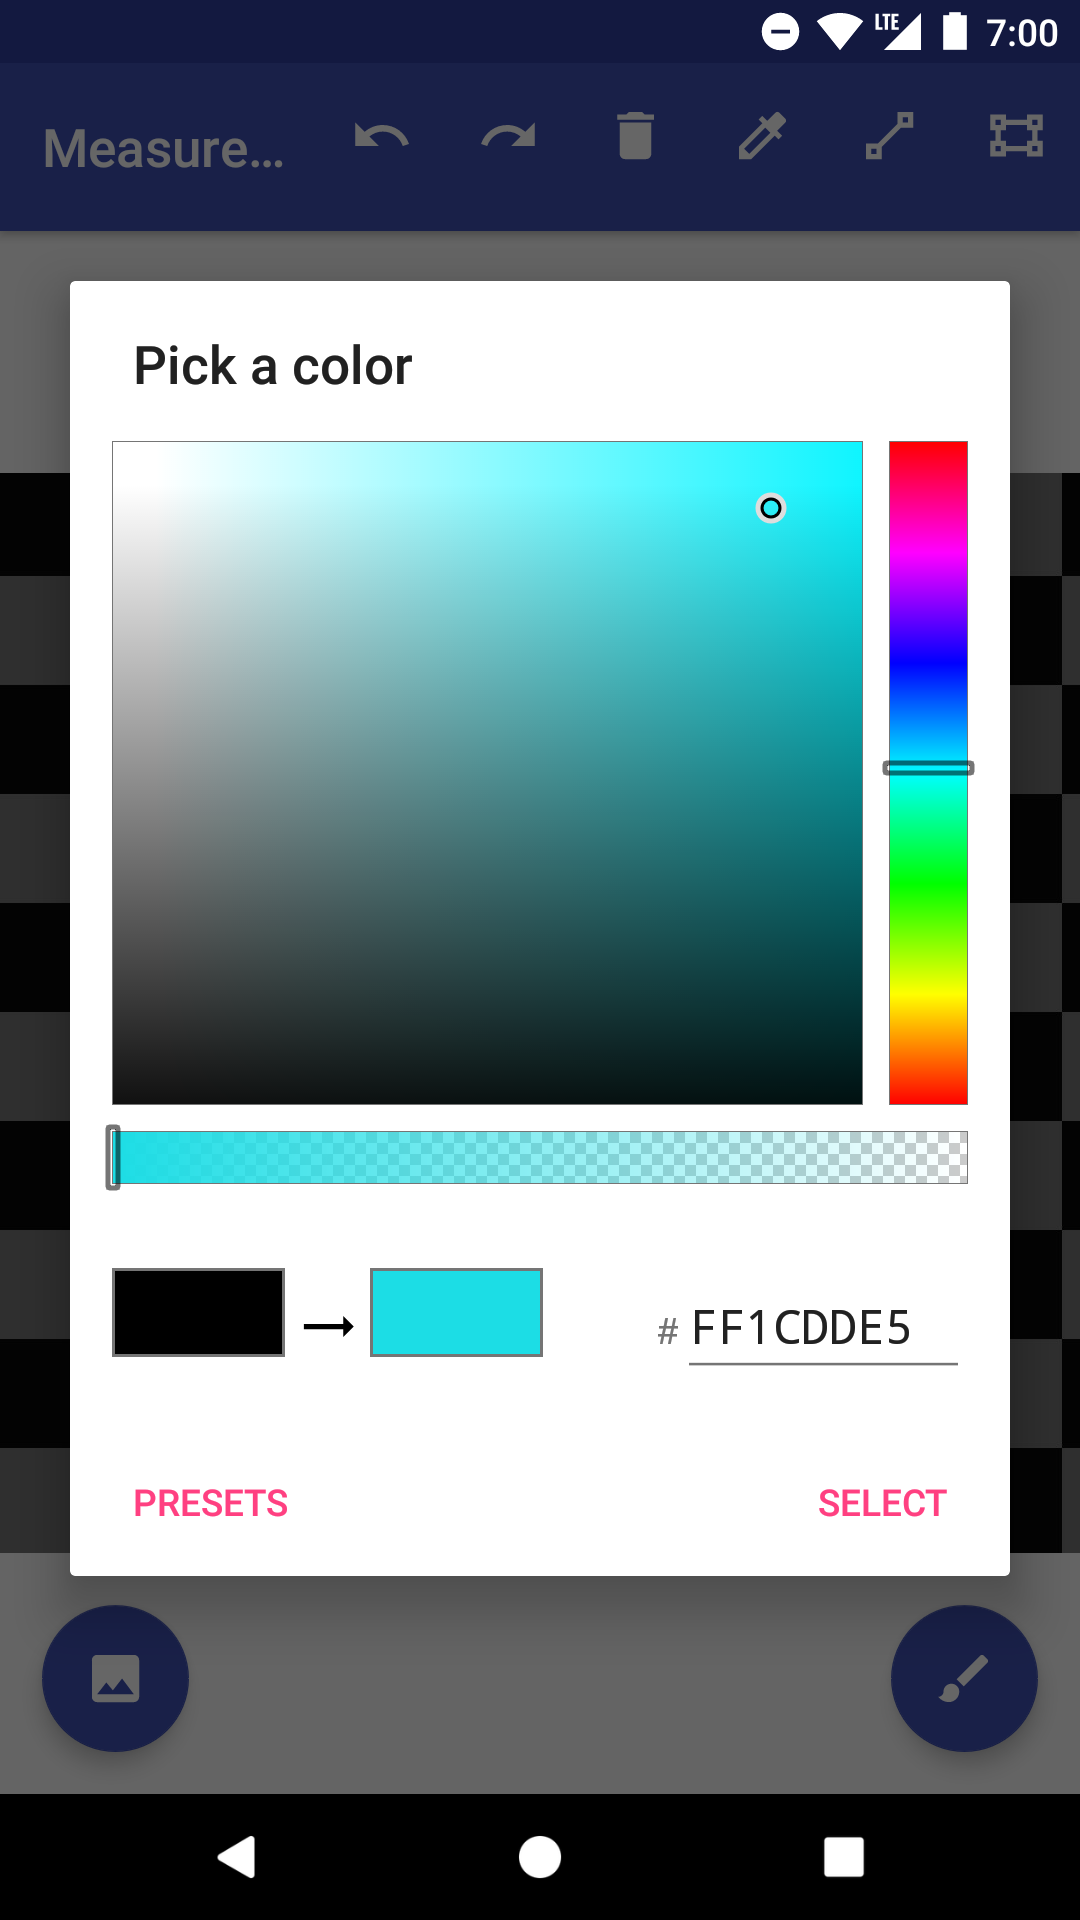
\includegraphics[keepaspectratio, width=0.4\textwidth]{prototype1/color}
  \caption{Geöffneter Farbauswahl-Dialog}
  \label{fig:color1}
\end{wrapfigure}

Des Weiteren wird die aktuell markierte Form im Zeichen-Modus durch graue Kreise an den Eckpunkten hervorgehoben, und zugleich soll dem Benutzer hierdurch verdeutlicht werden, dass mit Hilfe dieser Kreise die Form in ihrer Größe und Lage bearbeitet werden kann. \\

Im Text-Modus bietet sich dem Benutzer die Möglichkeit, Kanten mittels eines Eingabe-Dialogs zu beschriften (siehe \autoref{fig:labeling1}).
Hierzu öffnet sich beim langen Klick auf eine Form im Text-Modus ein modaler Dialog, welcher die Messwerte des Nutzers entgegennimmt.
Eingetragene Messwerte werden anschließend neben der zuvor ausgewählten Kante im Bild dargestellt (siehe \autoref{fig:label1}). \todo{neues Bild wo Messwert besser sichtbar}

\begin{figure}[h]
  \begin{subfigure}[t]{0.4\textwidth}
    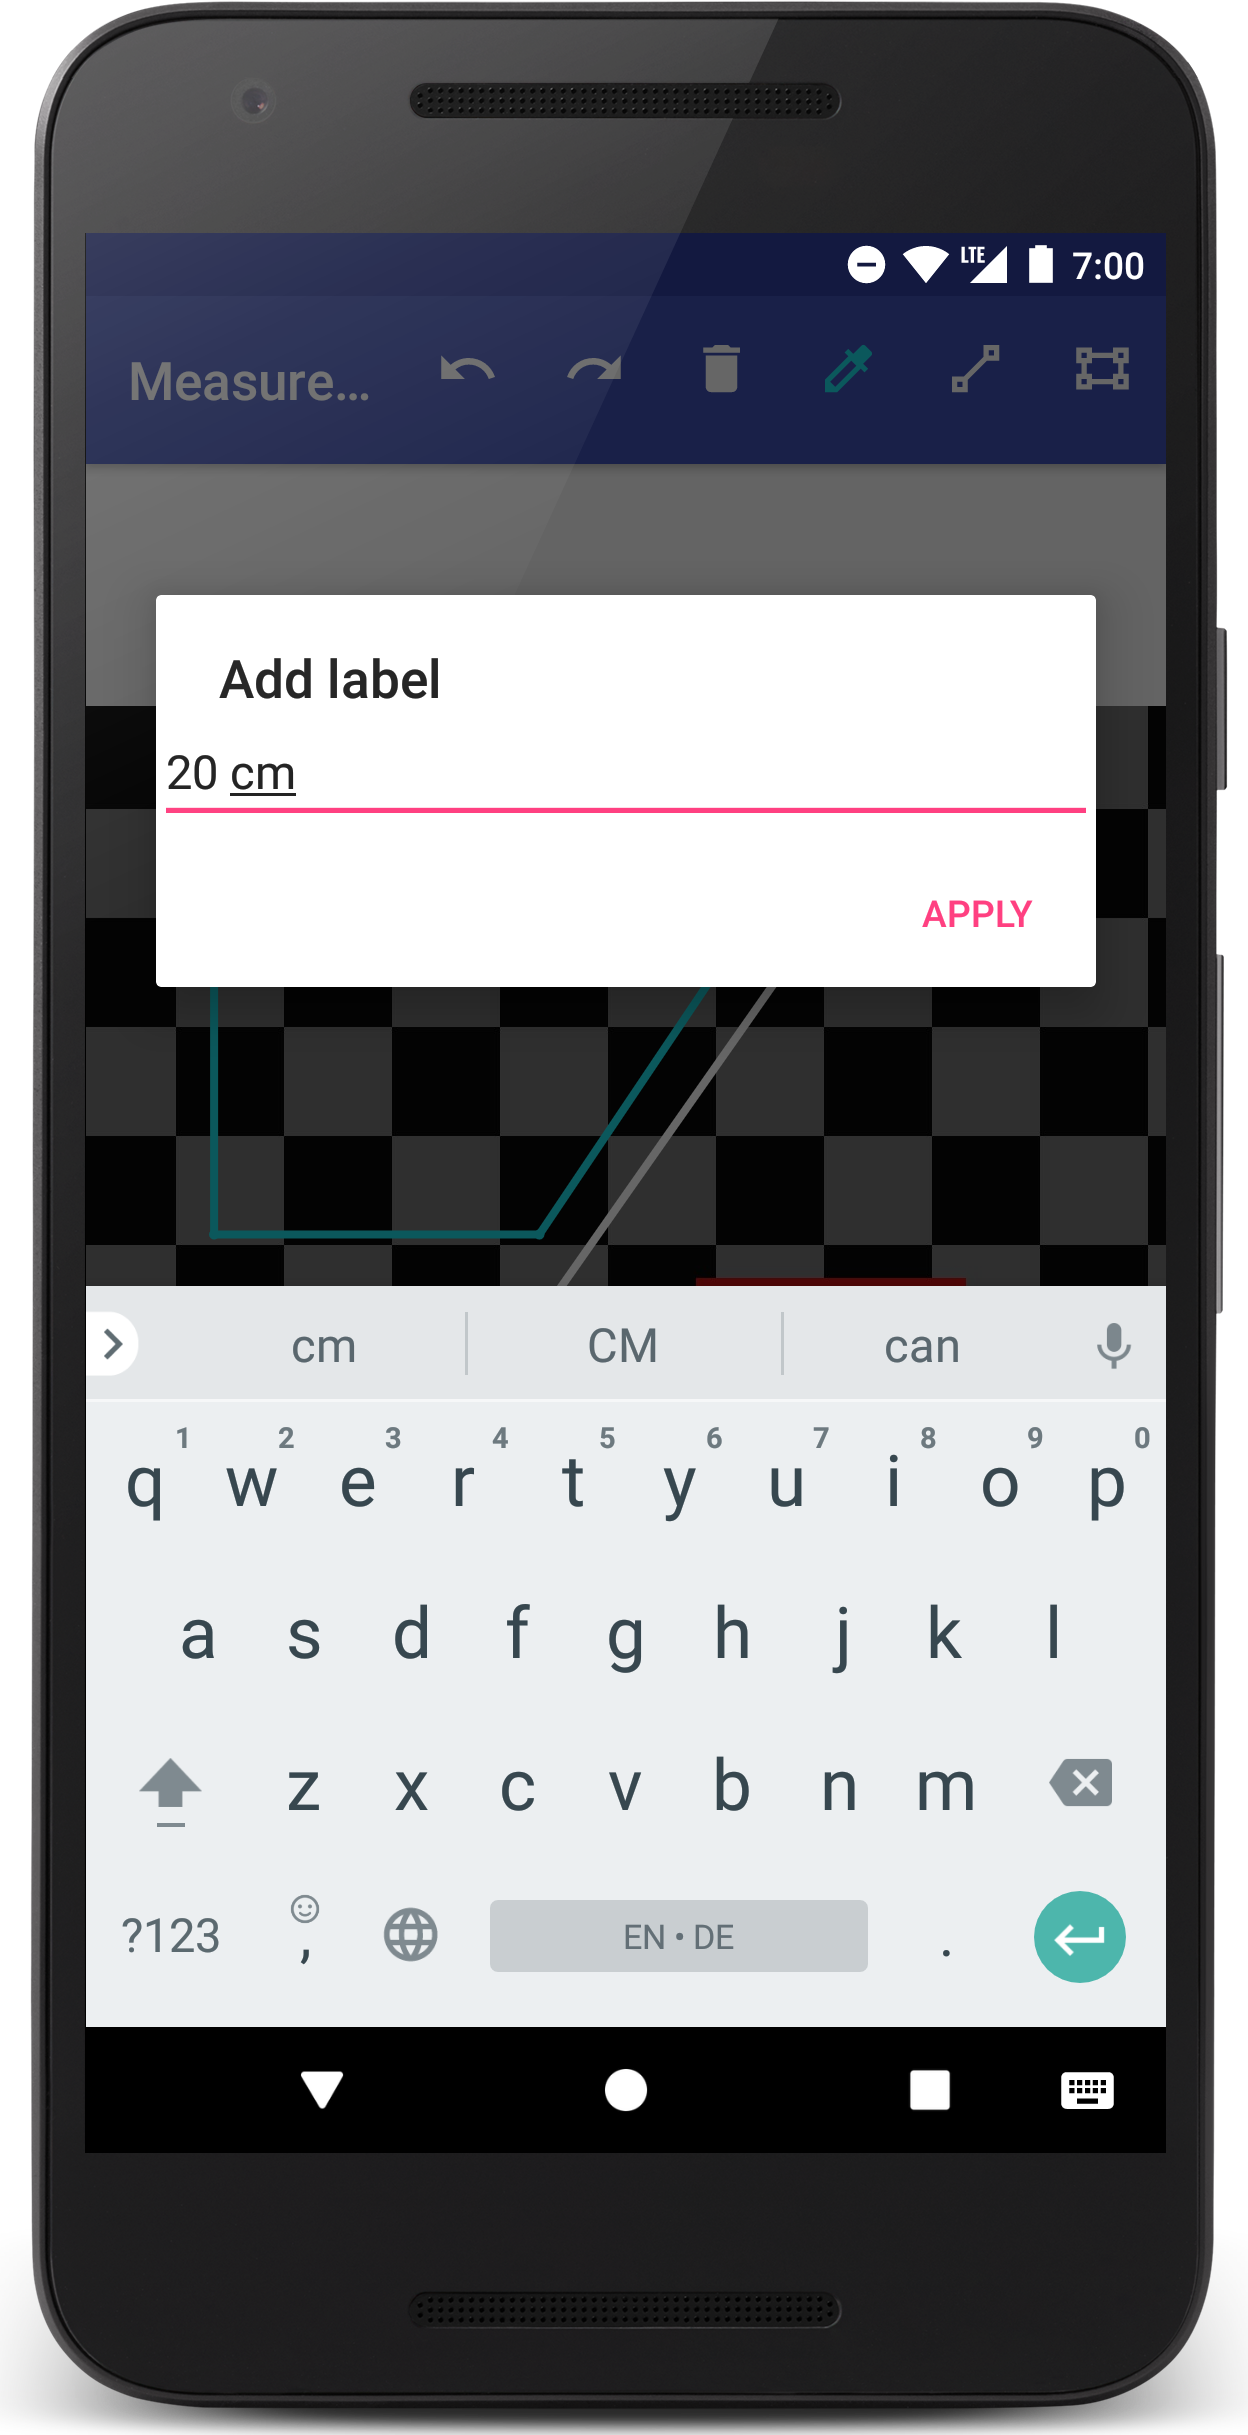
\includegraphics[keepaspectratio, width=\textwidth]{prototype1/labeling}
    \caption{Dialog zum Eintragen von Messwerten}
    \label{fig:labeling1}
  \end{subfigure}
  \begin{subfigure}[t]{0.4\textwidth}
    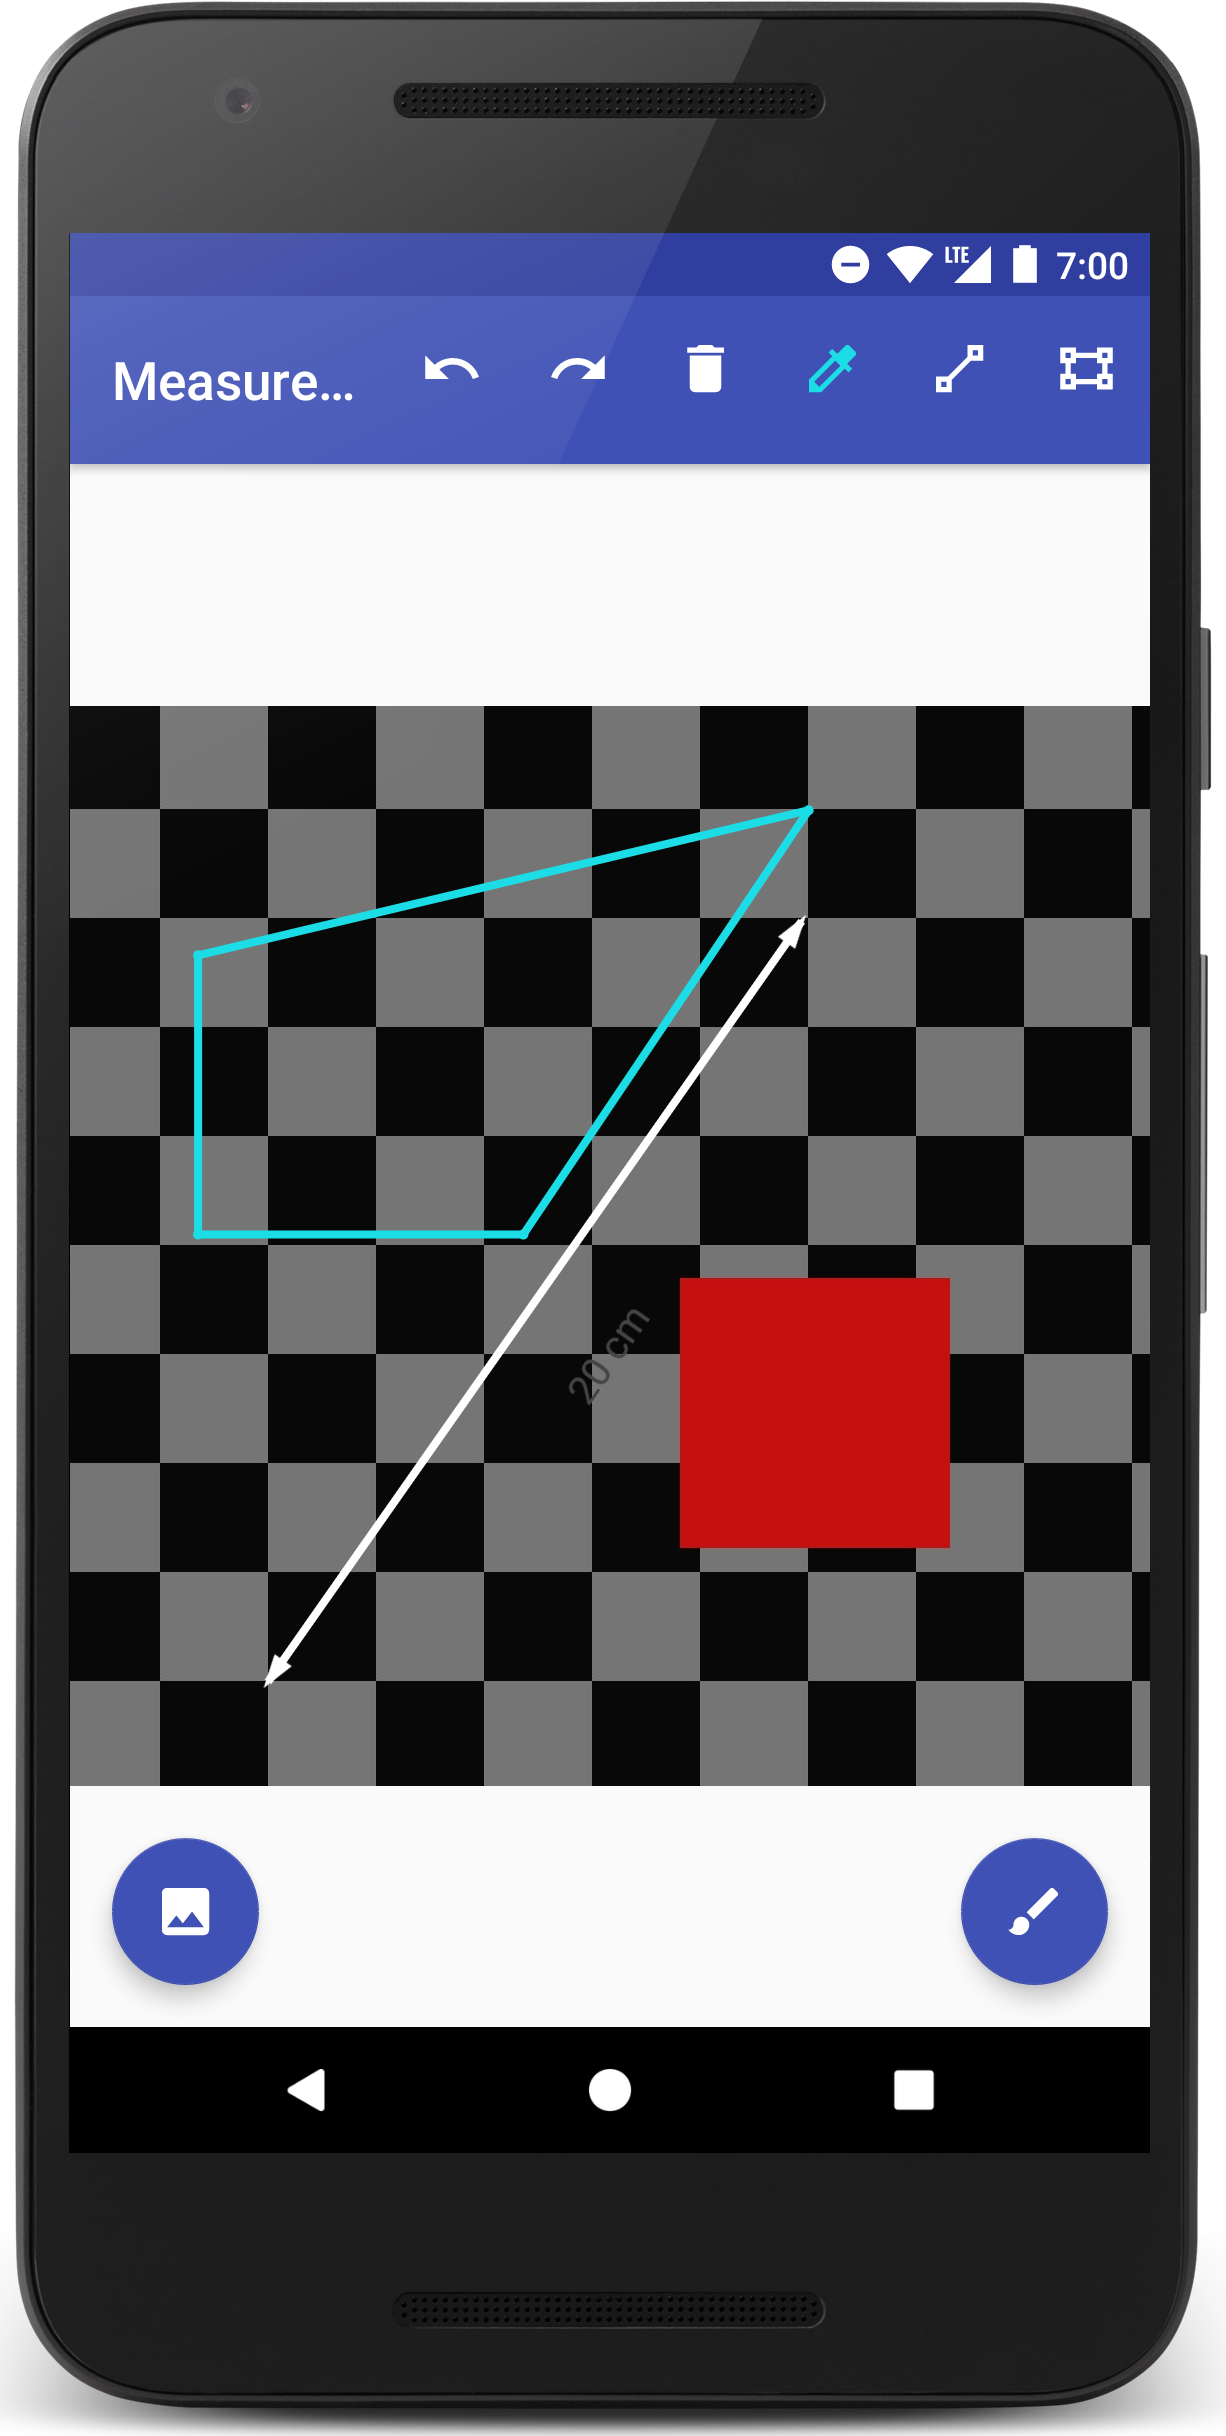
\includegraphics[keepaspectratio, width=\textwidth]{prototype1/label}
    \caption{Linie mit eingetragenem Messwert}
    \label{fig:label1}
  \end{subfigure}
  \centering
  \caption{Eintragen und Anzeigen von Messwerten im ersten Prototyp}
\end{figure}

\subsection{Rollout und Test}\label{subsec:test1}
Nachdem die App zwei Tage in den Arbeitsalltag der beiden Geschäftsführer der Fa. VERO integriert und währenddessen getestet wurde, gab es am 18. Dezember Feedback zur Implementierung des ersten Prototyps. \\

Nach Aussage beider Testpersonen, haben die \emph{Floating Action Buttons} sich bei der Benutzung der App als großes Hindernis herausgestellt.
So sei nicht intuitiv klar, dass die App über zwei verschiedene Modi, nämlich den Zeichen- und Text-Modus, verfügt.
Zudem sei unklar, dass man über einen Klick auf den rechten \emph{Floating Action Button} zwischen den beiden Modi hin und her wechseln könne. \\

Ein weiteres Problem ergab sich laut Testpersonen X \todo{Wie hier differenzieren?} bei der Benutzung der App auf seinem Tablet.
So seien sämtliche Texte nur schwer lesbar, und diverse Punkte zum Verändern der Formen zu klein, sodass sie nur mühsam und mit viel Konzentration mit dem Finger zu treffen seien. \\

Ein weiteres Problem, was beide Testpersonen schilderten, war die schlechte Lesbarkeit von eingetragenen Messwerten auf Bildern, die in dunkleren Lichtverhältnissen aufgenommen wurden.
Hier setze sich die Textfarbe zu schlecht vom Hintergrund ab. \\

Des Weiteren kam von beiden Testpersonen der Wunsch nach der Möglichkeit, Formen mit bereits vorhandenen Gerüsttypen wie zum Beispiel ``Hängegerüst'' oder ``Standgerüst'' zu verbinden, und in den Meta-Daten des Bildes zu speichern. \\

Außerdem wurde von beiden Testpersonen mehrfach angemerkt, dass es wünschenswert wäre, Bilder vor dem Bearbeiten über eine weitere Oberfläche zunächst zurecht zu schneiden und eventuell drehen zu können.
Dies sei eine essentielle Funktion, da es auf der Baustelle oftmals dazu komme, dass aufgenommene Bilder nicht nur das gewünschte Gerüst, sondern noch andere Objekte, die nicht relevant für das Bild seien, beinhalten. \\

Ursachen und mögliche Lösungsideen dieser Probleme sollen im nächsten Abschnitt in einer weiteren Iteration des ``Human-Centered Design Process' weiter ausgewertet und mit Hilfe eines zweiten Prototyps - bestenfalls optimal - gelöst werden.
